% !TeX root = main.tex

\section{实验结果}

本次实验用到的试块配合比可以从表~\ref{tab:proportion}中获取. 

\subsection{密度, 流动度, 抗压强度}

我们利用不锈钢密度杯与锥模测定了水泥净浆的密度与流动度, 并在 \SI{7}{\day} 后使用 \SI{300}{\kilo\newton} 试金试验机进行水泥净浆试块抗压强度试验. 结果如表~\ref{tab:density}所示. 

\begin{table}[!t]
  \centering
  \caption{水泥净浆密度, 流动度与水泥试块 \SI{7}{\day} 平均抗压强度实验结果}
  \resizebox{\linewidth}{!}{
  \begin{tabular}{ccccccccc}
    \toprule
    实验编号 & 粉煤灰掺量        & 水胶比    & 水泥 (\unit{\gram}) & 水 (\unit{\gram}) & 粉煤灰 (\unit{\gram}) & 密度 (\unit{\gram\per\centi\meter\cubed}) & 流动度 (\unit{\milli\meter}) & 平均抗压强度 (\unit{\mega\pascal}) \\
    \midrule
    1        & \SI{0}{\percent}  & \num{0.4} & \num{700}           & \num{280}         & \num{0}               & \num{1.935}                               & \num{133}          & \num{47.3}          \\
    2        & \SI{15}{\percent} & \num{0.4} & \num{595}           & \num{280}         & \num{105}             & \num{1.925}                               & \num{121}          & \num{37.8}          \\
    3        & \SI{30}{\percent} & \num{0.4} & \num{490}           & \num{280}         & \num{210}             & \num{1.882}                               & \num{117}          & \num{30.6}          \\
    \bottomrule
  \end{tabular}
  }
  \label{tab:density}
\end{table}

根据表~\ref{tab:density}, 我们可以发现以下几点:
\begin{itemize}
  \item 水泥净浆密度随着粉煤灰掺量的增加而降低, 这可能是因为粉煤灰的密度低于水泥的密度.
  \item 流动度随着粉煤灰掺量的增加而降低, 这可能是因为粉煤灰的比表面积大于水泥的比表面积, 增加了水泥净浆的黏度.
  \item 水泥试块 \SI{7}{\day} 抗压强度随着粉煤灰掺量的增加而降低, 这可能是因为粉煤灰的水化反应 (火山灰反应) 速度慢于水泥的水化反应速度, 导致早期强度下降.
\end{itemize}

\subsection{微观结构, 能谱图, 元素组成及成分分析}

\subsubsection{实验理论}
本实验的理论内容如下所示, 硬化水泥石中包含水泥水化产物\ce{Ca(OH)2}, \ce{CSH}, \ce{AFt}, 可能包含未水化的\ce{C2S}与\ce{C3S}. 在加入粉煤灰的水泥石中应该包含不参与反应的粉煤灰.

\begin{center}
  水化过程:

  石膏水化(放热反应):\ce{CaSO4*0.5H2O + 1.5H2O -> CaSO4*2H2O}

  \ce{C3A}水化:\ce{C3A + 10H -> C4AH10}
  
  \vspace{+1.em}
  \ce{C3A}与石膏反应(控制凝结硬化):

  \ce{C3A + 3C\overline{S}.H2 + 26H -> C3A*3C\overline{S}.H32}
  
  \vspace{+1.em}
  \ce{C3S}水化(控制早期、后期强度):
  
  \ce{2C3S + 6H -> C3S2H3 + 3CH}
  
  \vspace{+1.em}
  \ce{C2S}水化(控制后期强度):
  
  \ce{2C2 + 4H -> C3S2H3 + CH}
  
  \vspace{+1.em}
  水化产物:

  钙矾石\ce{AFt}、\ce{AFm}(体积15-20\%):决定混凝土的凝结

  氢氧化钙\ce{CH}(体积20-25\%):提供混凝土碱性、钢筋钝化延缓锈蚀

  水化硅酸钙凝胶\ce{CSH}(体积50-60\%):提供混凝土强度、抗渗性、体积稳定性、耐久性

\end{center}

\subsubsection{未水化的\ce{C3S}}
\begin{minipage}{\textwidth}
  \begin{minipage}[b]{0.32\textwidth}
    \centering
    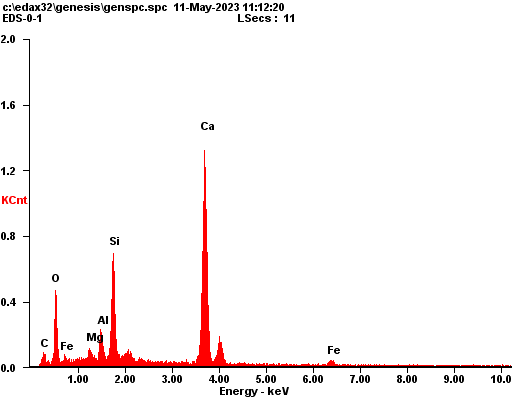
\includegraphics[width = \linewidth]{assets/spectrum/00-01-10000x-ETD-C3S.png}
    \captionof{figure}{粉煤灰掺量0\%, 01区域的能谱图}
  \end{minipage}
  \hfill
  \begin{minipage}[b]{0.32\textwidth}
    \centering
    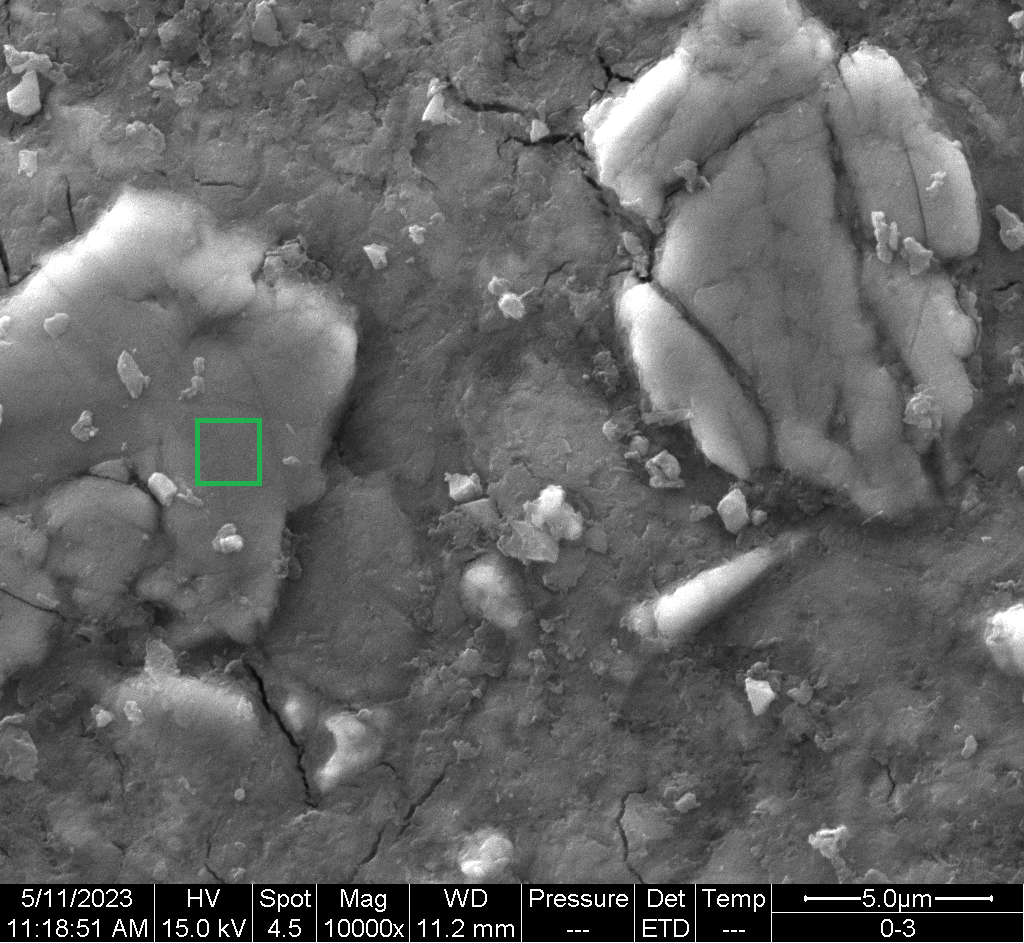
\includegraphics[width = \linewidth]{assets/spectrum selection/00-01-10000x-ETD-C3S.png}
    \captionof{figure}{粉煤灰掺量0\%, 01区域的ETD图像及选择区域}
    \label{fig:00-01-select}
  \end{minipage}
  \hfill
  \begin{minipage}[b]{0.32\textwidth}
    \centering
    \begin{tabular}{|c|c|c|}
      \hline
      Element & Wt \% & At \% \\ \hline
      C K     & 03.23 & 06.95 \\ \hline
      O K     & 27.17 & 43.92 \\ \hline
      MgK     & 01.58 & 01.69 \\ \hline
      AlK     & 03.04 & 02.92 \\ \hline
      SiK     & 12.12 & 11.16 \\ \hline
      CaK     & 48.70 & 31.43 \\ \hline
      FeK     & 04.16 & 01.93 \\ \hline
    \end{tabular}
    \captionof{table}{粉煤灰掺量0\%, 01区域的元素组成}
    \label{tab:00-01}
  \end{minipage}
\end{minipage}

\begin{minipage}{\textwidth}
  \begin{minipage}[b]{0.32\textwidth}
    \centering
    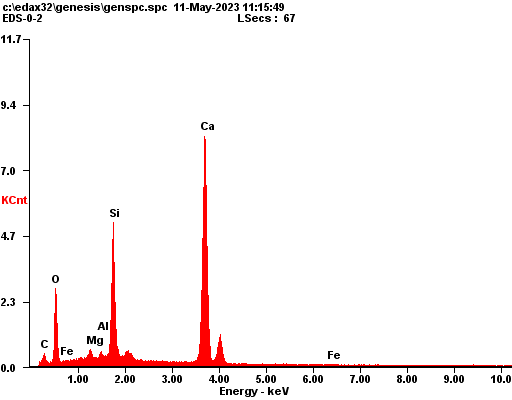
\includegraphics[width = \linewidth]{assets/spectrum/00-02-10000x-ETD-C3S.png}
    \captionof{figure}{粉煤灰掺量0\%, 02区域的能谱图}
  \end{minipage}
  \hfill
  \begin{minipage}[b]{0.32\textwidth}
    \centering
    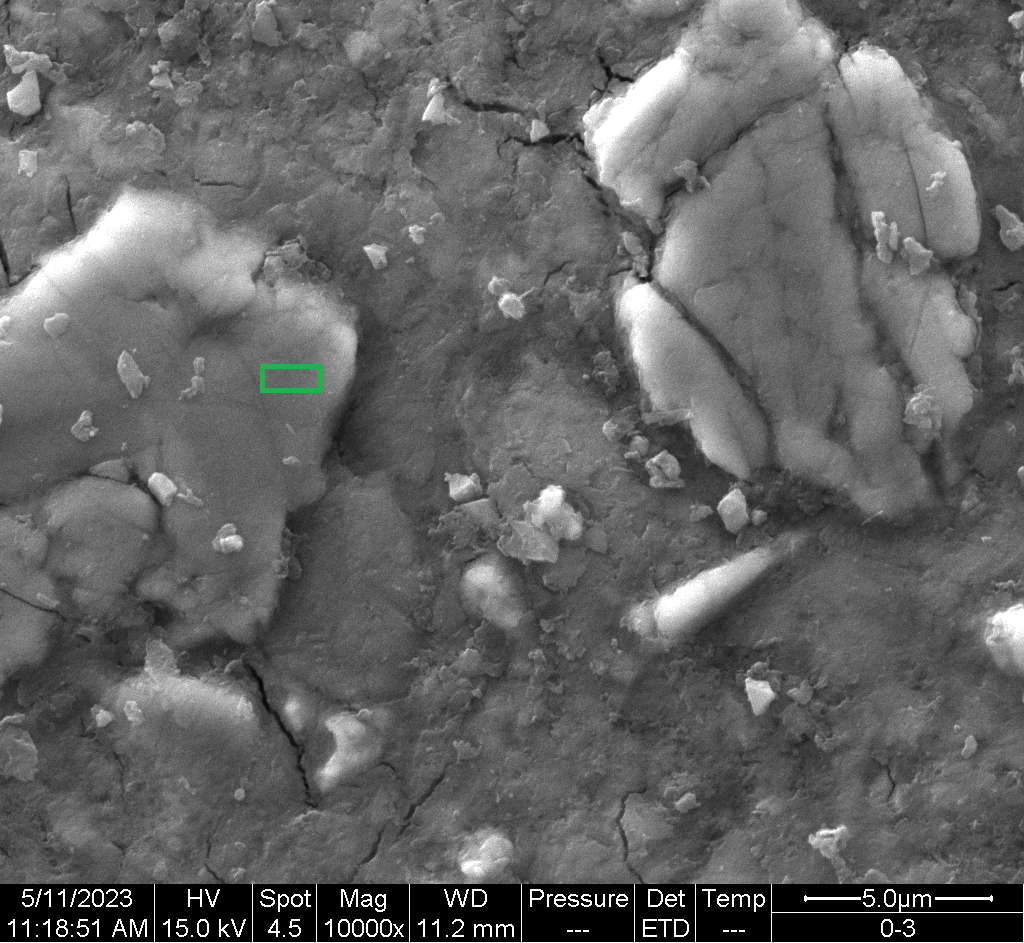
\includegraphics[width = \linewidth]{assets/spectrum selection/00-02-10000x-ETD-C3S.png}
    \captionof{figure}{粉煤灰掺量0\%, 02区域的ETD图像及选择区域}
    \label{fig:00-02-select}
  \end{minipage}
  \hfill
  \begin{minipage}[b]{0.32\textwidth}
    \centering
    \begin{tabular}{|c|c|c|}
      \hline
      Element & Wt \% & At \% \\ \hline
      C K     & 02.69 & 05.74 \\ \hline
      O K     & 28.78 & 46.18 \\ \hline
      MgK     & 00.96 & 01.01 \\ \hline
      AlK     & 00.42 & 00.40 \\ \hline
      SiK     & 13.88 & 12.69 \\ \hline
      CaK     & 52.52 & 33.63 \\ \hline
      FeK     & 00.75 & 00.35 \\ \hline
    \end{tabular}
    \captionof{table}{粉煤灰掺量0\%, 02区域的元素组成}
    \label{tab:00-02}
  \end{minipage}
\end{minipage}

在ETD图像中发现了如图~\ref{fig:00-01-select}与图~\ref{fig:00-02-select}的微观结构, 选择以上微观结构区域进行能谱分析, 结果分别如表~\ref{tab:00-01}与表~\ref{tab:00-02}所示. 在表格中, 我们发现\ce{Ca}与\ce{Si}的物质的量之比大约为3:1, 考虑钙, 硅的物质的量之比, 该区域成分应该是\ce{C3S}.

\subsubsection{未水化的\ce{C2S} }

\begin{minipage}{\textwidth}
  \begin{minipage}[b]{0.32\textwidth}
    \centering
    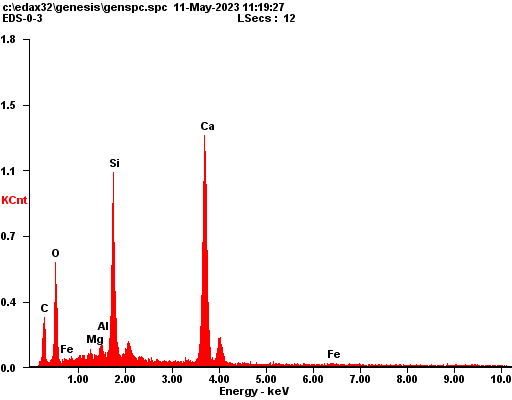
\includegraphics[width = \linewidth]{assets/spectrum/00-03-15000x-ETD-C2S.png}
    \captionof{figure}{粉煤灰掺量0\%, 03区域的能谱图}
  \end{minipage}
  \hfill
  \begin{minipage}[b]{0.32\textwidth}
    \centering
    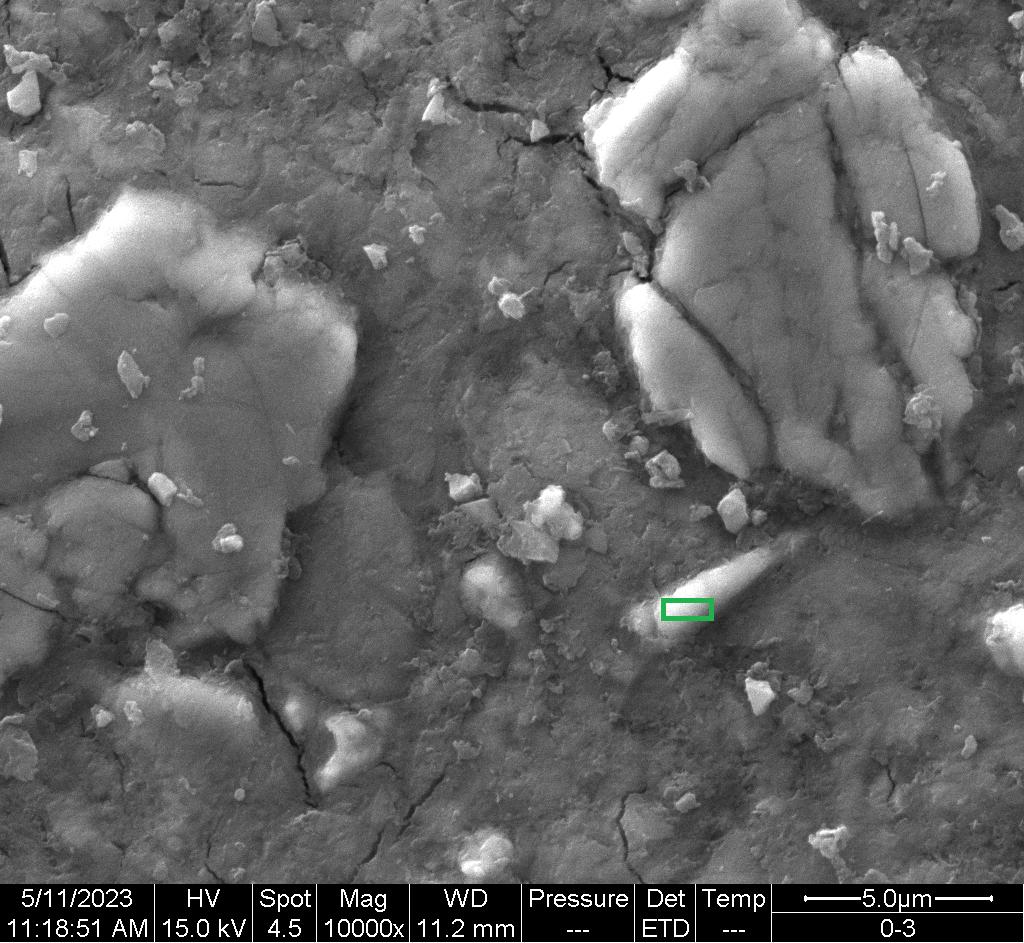
\includegraphics[width = \linewidth]{assets/spectrum selection/00-03-10000x-ETD-C2S.png}
    \captionof{figure}{粉煤灰掺量0\%, 03区域的ETD图像及选择区域}
    \label{fig:00-03-select}
  \end{minipage}
  \hfill
  \begin{minipage}[b]{0.32\textwidth}
    \centering
    \begin{tabular}{|c|c|c|}
      \hline
      Element & Wt \% & At \% \\ \hline
      C K     & 10.18 & 19.55 \\ \hline
      O K     & 28.70 & 41.35 \\ \hline
      MgK     & 00.45 & 00.43 \\ \hline
      AlK     & 00.94 & 00.80 \\ \hline
      SiK     & 14.96 & 12.28 \\ \hline
      CaK     & 43.80 & 25.19 \\ \hline
      FeK     & 00.96 & 00.40 \\ \hline
    \end{tabular}
    \captionof{table}{粉煤灰掺量0\%, 03区域的元素组成}
    \label{tab:00-03}
  \end{minipage}
\end{minipage}

在ETD图像中发现了如图~\ref{fig:00-03-select}的微观结构, 选择以上微观结构区域进行能谱分析, 结果分别如表~\ref{tab:00-03}所示. 在表格中, 我们发现\ce{Ca}与\ce{Si}的物质的量之比大约为2:1, 考虑钙, 硅的物质的量之比, 该区域成分应该是\ce{C2S}.

\subsubsection{水化产物\ce{CH} 或 \ce{Ca(OH)2} }

\begin{minipage}{\textwidth}
  \begin{minipage}[b]{0.32\textwidth}
    \centering
    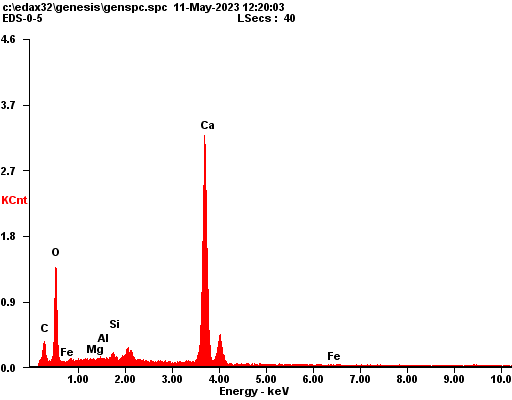
\includegraphics[width = \linewidth]{assets/spectrum/00-05-10000x-ETD-CH.png}
    \captionof{figure}{粉煤灰掺量0\%, 05区域的能谱图}
  \end{minipage}
  \hfill
  \begin{minipage}[b]{0.32\textwidth}
    \centering
    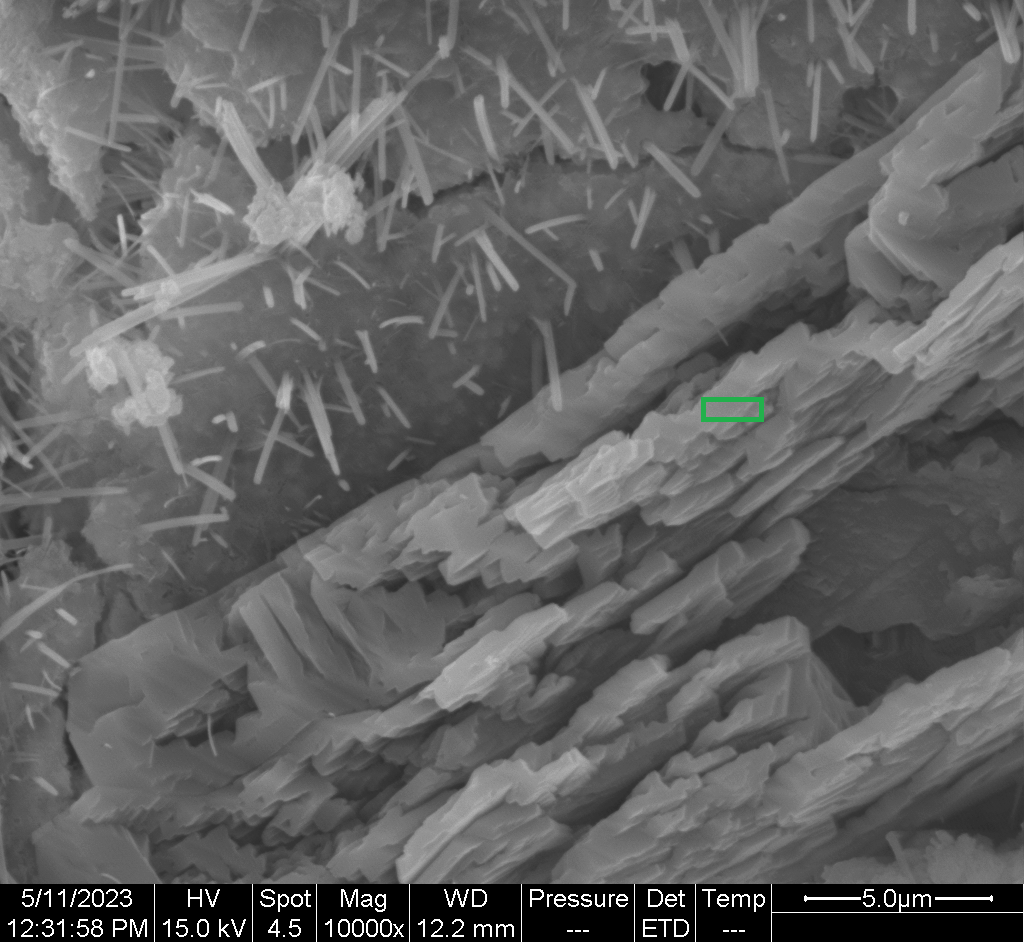
\includegraphics[width = \linewidth]{assets/spectrum selection/00-05-10000x-ETD-CH.png}
    \captionof{figure}{粉煤灰掺量0\%, 05区域的ETD图像及选择区域}
    \label{fig:00-05-select}
  \end{minipage}
  \hfill
  \begin{minipage}[b]{0.32\textwidth}
    \centering
    \begin{tabular}{|c|c|c|}
      \hline

      Element & Wt \% & At \% \\ \hline
      C K     & 02.24 & 05.37 \\ \hline
      O K     & 22.10 & 39.79 \\ \hline
      MgK     & 00.30 & 00.36 \\ \hline
      AlK     & 00.41 & 00.44 \\ \hline
      SiK     & 00.90 & 00.93 \\ \hline
      CaK     & 73.53 & 52.85 \\ \hline
      FeK     & 00.52 & 00.27 \\ \hline
    \end{tabular}
    \captionof{table}{粉煤灰掺量0\%, 05区域的元素组成}
    \label{tab:00-05}
  \end{minipage}
\end{minipage}

\begin{minipage}{\textwidth}
  \begin{minipage}[b]{0.32\textwidth}
    \centering
    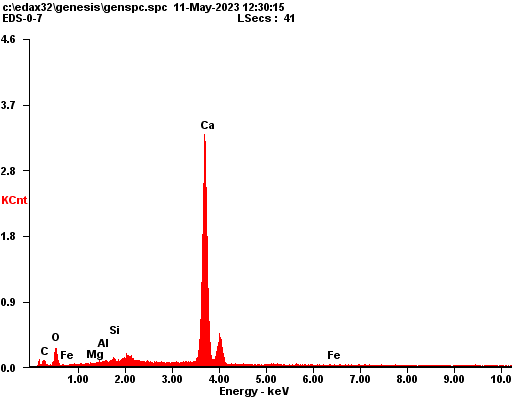
\includegraphics[width = \linewidth]{assets/spectrum/00-07-10000x-ETD-CH.png}
    \captionof{figure}{粉煤灰掺量0\%, 07区域的能谱图}
  \end{minipage}
  \hfill
  \begin{minipage}[b]{0.32\textwidth}
    \centering
    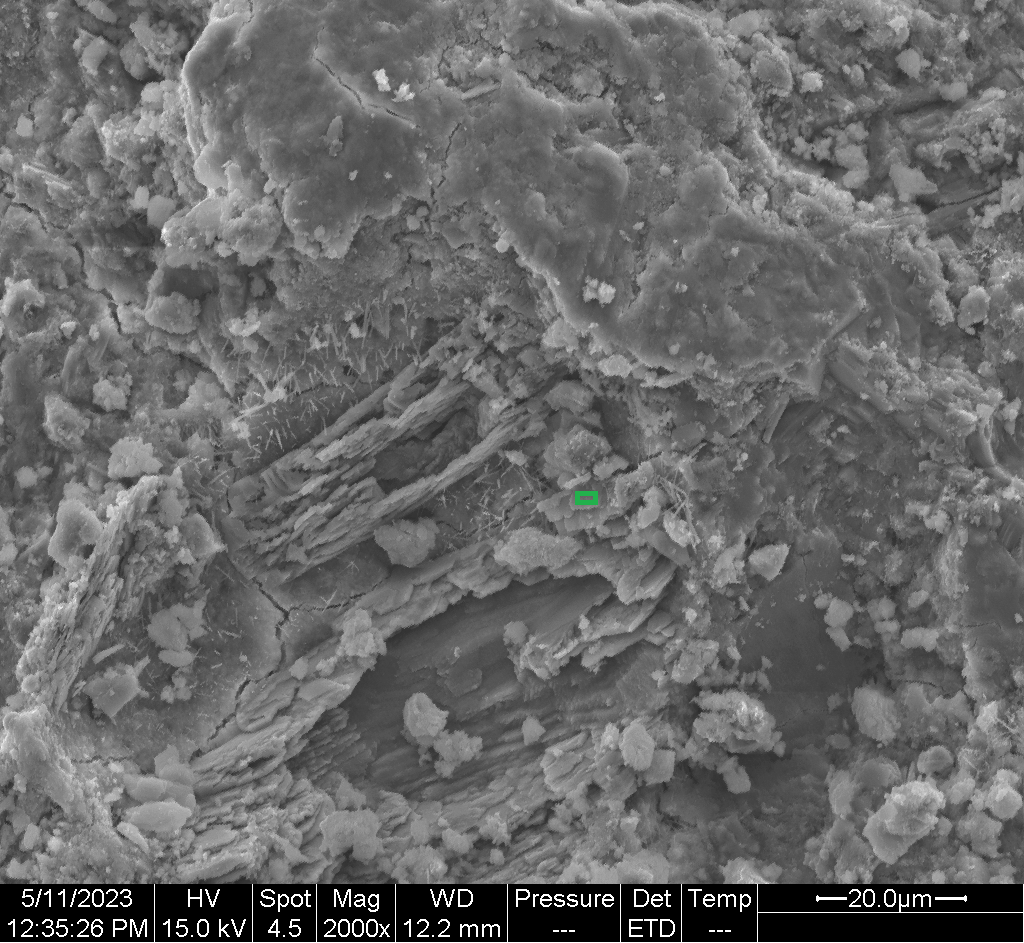
\includegraphics[width = \linewidth]{assets/spectrum selection/00-07-02000x-ETD-CH.png}
    \captionof{figure}{粉煤灰掺量0\%, 07区域的ETD图像及选择区域}
    \label{fig:00-07-select}
  \end{minipage}
  \hfill
  \begin{minipage}[b]{0.32\textwidth}
    \centering
    \begin{tabular}{|c|c|c|}
      \hline
      Element & Wt \% & At \% \\ \hline
      C K     & 01.37 & 03.63 \\ \hline
      O K     & 14.85 & 29.56 \\ \hline
      MgK     & 00.11 & 00.15 \\ \hline
      AlK     & 00.34 & 00.40 \\ \hline
      SiK     & 00.86 & 00.98 \\ \hline
      CaK     & 81.36 & 64.65 \\ \hline
      FeK     & 01.09 & 00.62 \\ \hline
    \end{tabular}
    \captionof{table}{粉煤灰掺量0\%, 07区域的元素组成}
    \label{tab:00-07}
  \end{minipage}
\end{minipage}

在ETD图像中发现了如图~\ref{fig:00-05-select}和图~\ref{fig:00-07-select}的片层状微观结构, 选择以上微观结构区域进行能谱分析, 结果分别如表~\ref{tab:00-05}和表~\ref{tab:00-07}所示. 在表格中, 我们发现在表格中主要的元素组成为\ce{Ca}与\ce{O}, 而\ce{Si}等其他元素很少, 推测该区域成分是\ce{CH}, 即\ce{Ca(OH)2}.

\subsubsection{水化产物\ce{CSH}}

\begin{minipage}{\textwidth}
  \begin{minipage}[b]{0.32\textwidth}
    \centering
    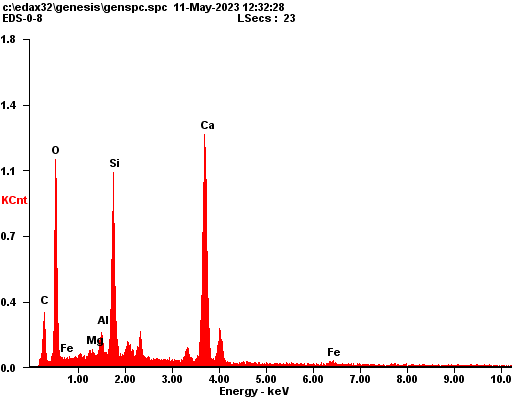
\includegraphics[width = \linewidth]{assets/spectrum/00-08-10000x-ETD-CSH.png}
    \captionof{figure}{粉煤灰掺量0\%, 08区域的能谱图}
  \end{minipage}
  \hfill
  \begin{minipage}[b]{0.32\textwidth}
    \centering
    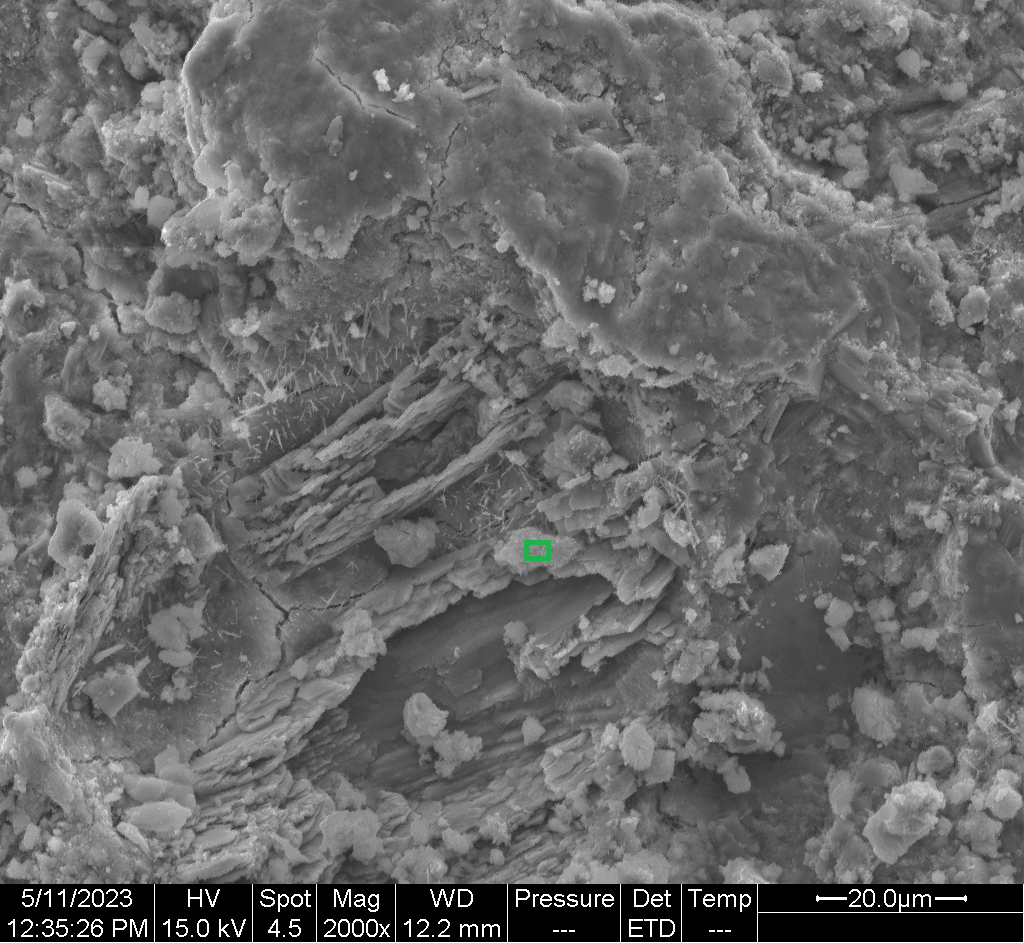
\includegraphics[width = \linewidth]{assets/spectrum selection/00-08-02000x-ETD-CSH.png}
    \captionof{figure}{粉煤灰掺量0\%, 08区域的ETD图像及选择区域}
    \label{fig:00-08-select}
  \end{minipage}
  \hfill
  \begin{minipage}[b]{0.32\textwidth}
    \centering
    \begin{tabular}{|c|c|c|}
      \hline
      Element & Wt \% & At \% \\ \hline
      C K     & 08.04 & 14.52 \\ \hline
      O K     & 40.04 & 54.29 \\ \hline
      MgK     & 00.48 & 00.43 \\ \hline
      AlK     & 01.49 & 01.20 \\ \hline
      SiK     & 12.39 & 09.57 \\ \hline
      CaK     & 35.43 & 19.17 \\ \hline
      FeK     & 02.13 & 00.83 \\ \hline
    \end{tabular}
    \captionof{table}{粉煤灰掺量0\%, 08区域的元素组成}
    \label{tab:00-08}
  \end{minipage}
\end{minipage}

\begin{minipage}{\textwidth}
  \begin{minipage}[b]{0.32\textwidth}
    \centering
    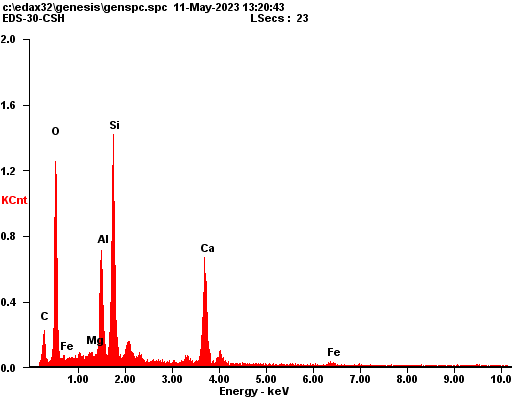
\includegraphics[width = \linewidth]{assets/spectrum/30-01-30000x-ETD-CSH.png}
    \captionof{figure}{粉煤灰掺量30\%, 01区域的能谱图}
  \end{minipage}
  \hfill
  \begin{minipage}[b]{0.32\textwidth}
    \centering
    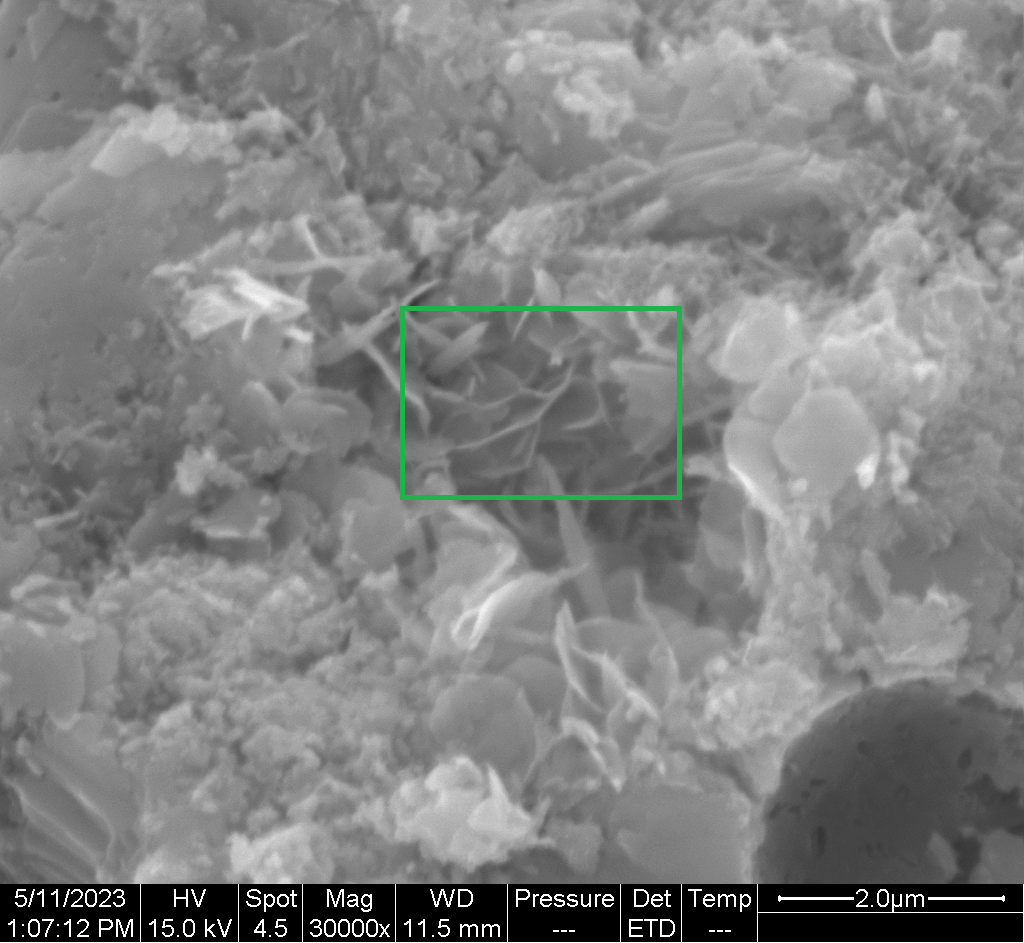
\includegraphics[width = \linewidth]{assets/spectrum selection/30-01-30000x-CSH.png}
    \captionof{figure}{粉煤灰掺量30\%, 01区域的ETD图像及选择区域}
    \label{fig:30-01-select}
  \end{minipage}
  \hfill
  \begin{minipage}[b]{0.32\textwidth}
    \centering
    \begin{tabular}{|c|c|c|}
      \hline
      Element & Wt \% & At \% \\ \hline
      C K     & 09.18 & 15.71 \\ \hline
      O K     & 40.78 & 52.38 \\ \hline
      MgK     & 00.43 & 00.36 \\ \hline
      AlK     & 08.57 & 06.53 \\ \hline
      SiK     & 19.82 & 14.50 \\ \hline
      CaK     & 18.75 & 09.61 \\ \hline
      FeK     & 02.47 & 00.91 \\ \hline
    \end{tabular}
    \captionof{table}{粉煤灰掺量30\%, 01区域的元素组成}
    \label{tab:30-01}
  \end{minipage}
\end{minipage}

在ETD图像中发现了如图~\ref{fig:00-08-select}和图~\ref{fig:30-01-select}的网络状微观结构, 选择以上微观结构区域进行能谱分析, 结果如表~\ref{tab:00-08}和表~\ref{tab:30-01}所示. 在图中, 我们发现该微观结构并没有规则的结构, 也不存在规律性, 因此排除其为晶体的可能性; 同时, 由于其体积尺寸超出\SI{10}{\micro\meter} , 因而推断其属于\ce{CSH}. 同时, 在表格中, 我们发现在表格中主要的元素组成为\ce{Ca}, \ce{Si} 与 \ce{O}, 且\ce{O} 元素成分极大, 推测该区域成分是\ce{CSH} 凝胶.
% 在ETD图像中发现了如图~\ref{fig:30-01-select}的网络状微观结构, 选择以上微观结构区域进行能谱分析, 结果如表~\ref{tab:30-01}所示. 在图中, 我们发现该微观结构并没有规则的结构, 也不存在规律性, 因此排除其为晶体的可能性; 同时, 由于其体积尺寸超出\SI{10}{\micro\meter} , 因而推断其属于\ce{CSH}. 同时, 在表格中, 我们发现在表格中主要的元素组成为\ce{Ca}, \ce{Si} 与 \ce{O}, 且\ce{O} 元素成分极大, 推测该区域成分是\ce{CSH} 凝胶.
\wei{最好对CSH做一些定量的分析, 通过其At\% 来分析. }

\begin{figure}
  \centering
  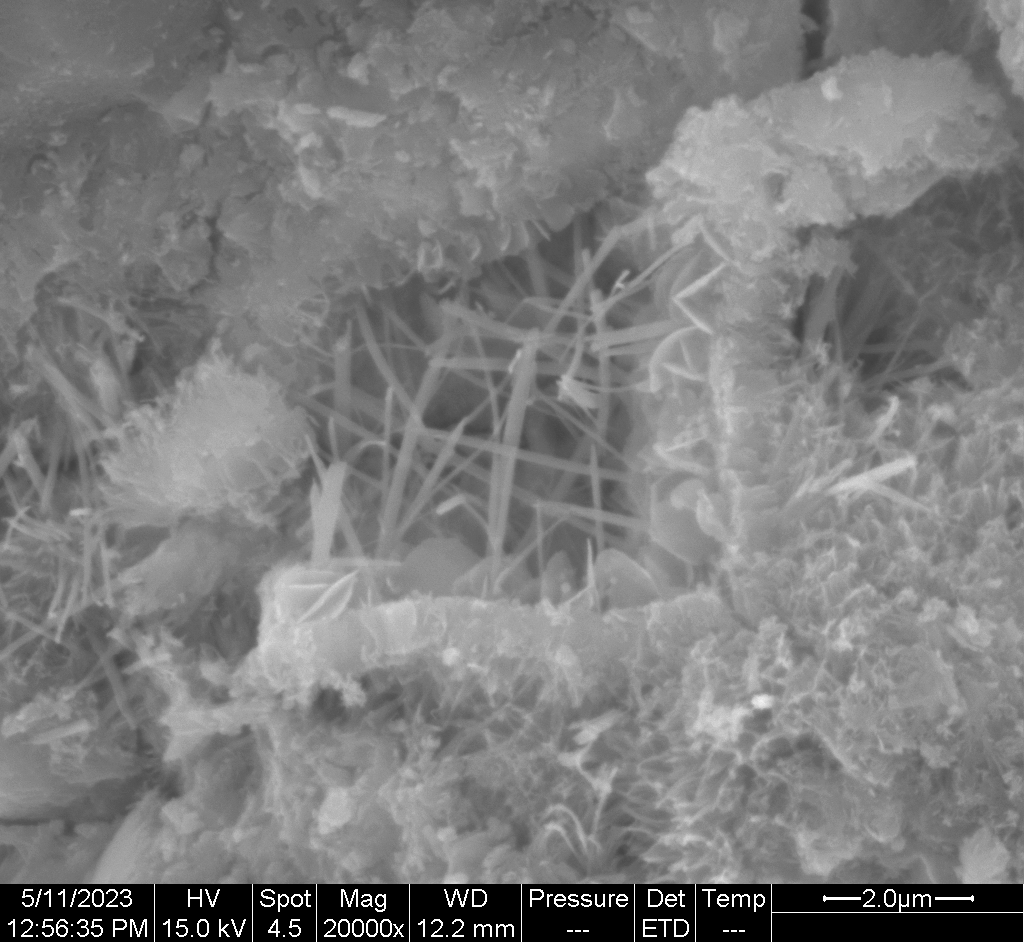
\includegraphics[width=0.5\textwidth]{assets/15-unpolished-20000x-ETD.png}
  \caption{粉煤灰掺量15\%, 未抛光的硬化水泥石, 在20000x倍率下的ETD图像. }
  \label{fig:ETD-CSH}
\end{figure}

更细致的网络结构如图~\ref{fig:ETD-CSH}所示.

\subsubsection{水化产物\ce{AFt}}

在ETD图像中发现了如图~\ref{fig:00-05-select}左上方所示的针棒状微观结构, 发现其微观结构规则, 认为其属于晶体; 考虑到其针棒状结构, 推测其属于钙矾石\ce{AFt}. 然而, 遗憾的是, 由于其分布区域过小, 无法选择区域对其做能谱分析, 进行验证.

\subsubsection{粉煤灰}\label{sec:fa}

\begin{minipage}{\textwidth}
  \begin{minipage}[b]{0.32\textwidth}
    \centering
    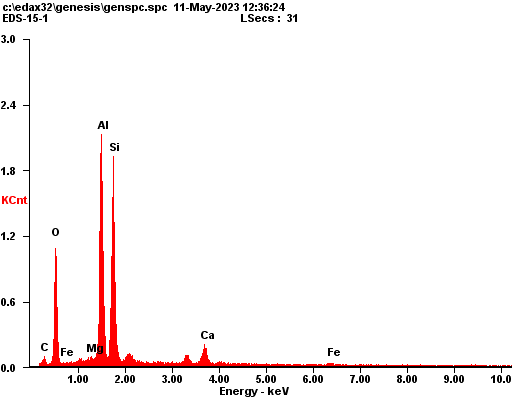
\includegraphics[width = \linewidth]{assets/spectrum/15-01-4000x-ETD-FA.png}
    \captionof{figure}{粉煤灰掺量15\%, 01区域的能谱图}
  \end{minipage}
  \hfill
  \begin{minipage}[b]{0.32\textwidth}
    \centering
    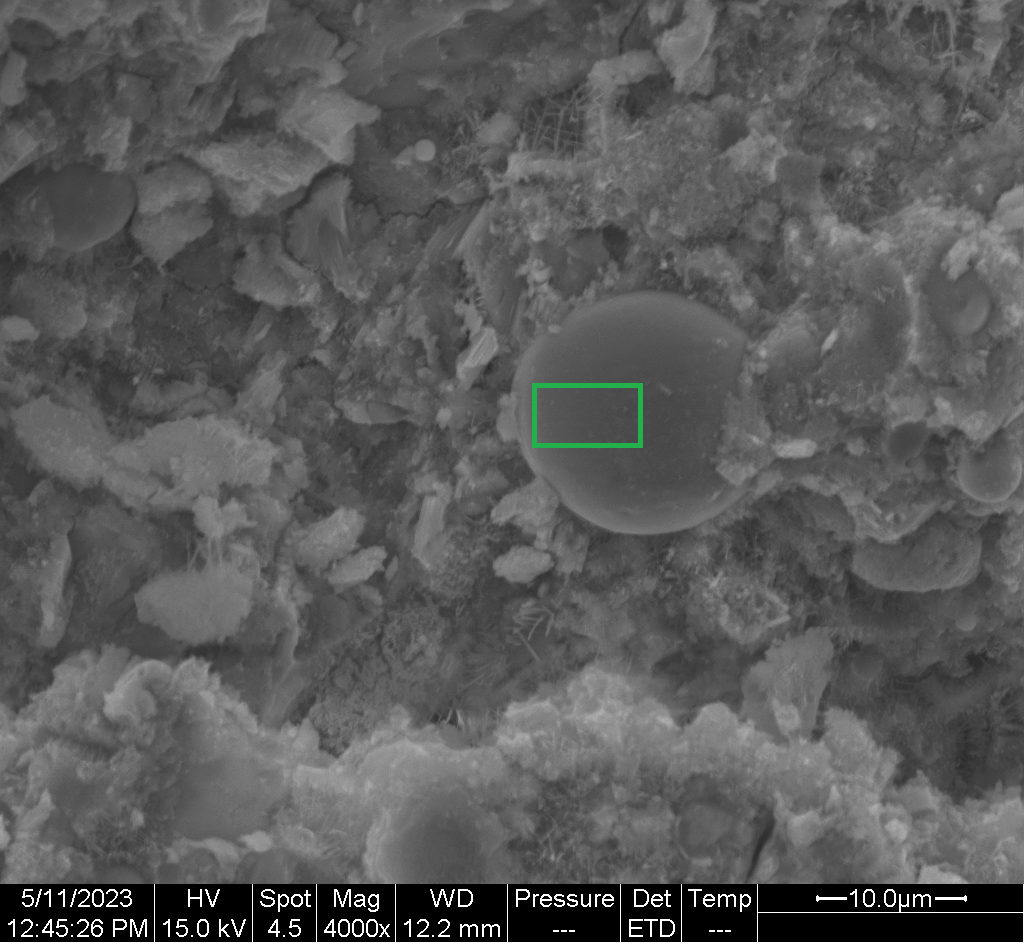
\includegraphics[width = \linewidth]{assets/spectrum selection/15-01-04000x-ETD-FA.png}
    \captionof{figure}{粉煤灰掺量15\%, 01区域的ETD图像及选择区域}
    \label{fig:15-01-select}
  \end{minipage}
  \hfill
  \begin{minipage}[b]{0.32\textwidth}
    \centering
    \begin{tabular}{|c|c|c|}
      \hline
      Element & Wt \% & At \% \\ \hline
      C K     & 05.53 & 10.11 \\ \hline
      O K     & 29.58 & 40.58 \\ \hline
      MgK     & 00.46 & 00.41 \\ \hline
      AlK     & 26.03 & 21.17 \\ \hline
      SiK     & 30.33 & 23.70 \\ \hline
      CaK     & 05.58 & 03.05 \\ \hline
      FeK     & 02.48 & 00.98 \\ \hline
    \end{tabular}
    \captionof{table}{粉煤灰掺量15\%, 01区域的元素组成}
    \label{tab:15-01}
  \end{minipage}
\end{minipage}

在ETD图像中发现了如图~\ref{fig:15-01-select}的球形的微观结构, 选择以上微观结构区域进行能谱分析, 结果如表~\ref{tab:15-01}所示. 我们发现在表格中主要的元素组成为\ce{Si}, \ce{Al} 与 \ce{O}, 且含有一定量的\ce{C} ; 而粉煤灰主要成分为粉煤灰主要成分是硅铝酸钙, 且钙的含量一般较低, 由于粉煤灰是火电厂的产品, 可能含有\ce{C}, 而且因而认为该区域成分是粉煤灰.

\begin{figure}[!t]
  \centering
  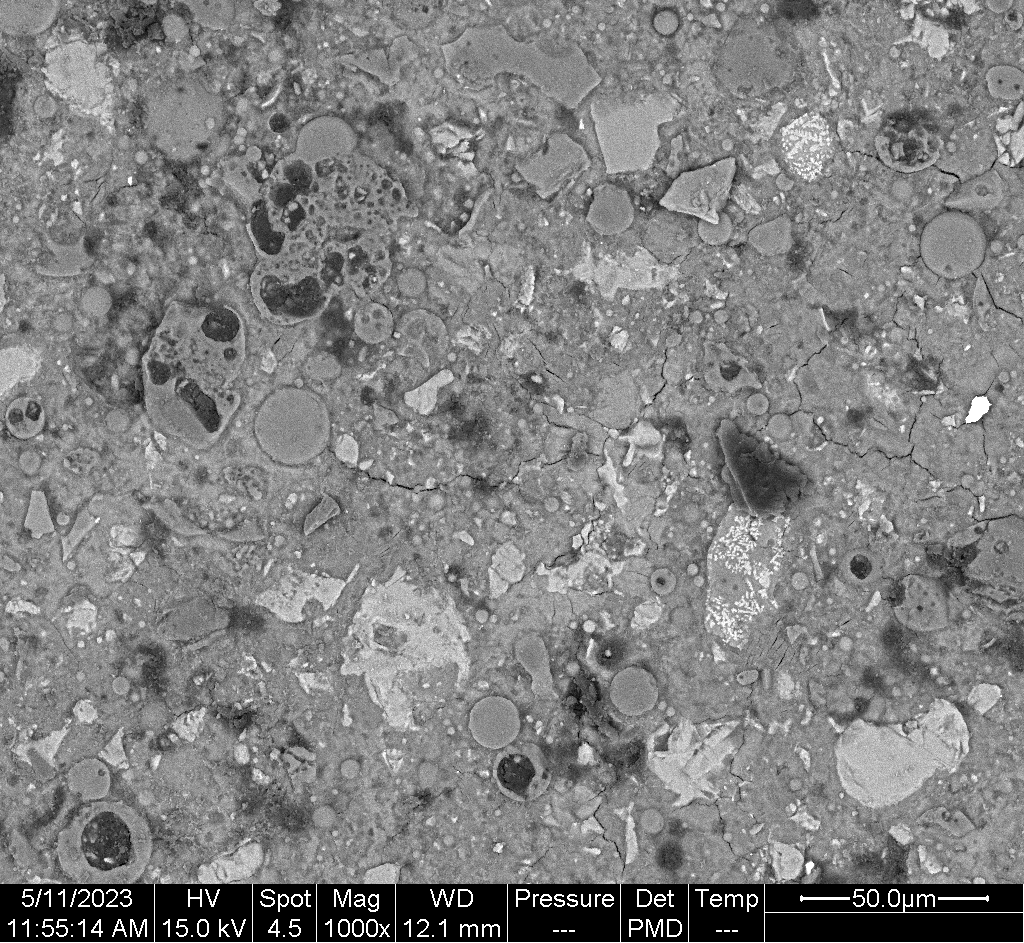
\includegraphics[width = 0.5\textwidth]{assets/30-polished-01000x-PMD.png}
  \caption{粉煤灰掺量30\%, 抛光后的硬化水泥块, 在1000x放大倍率下的背散射图. }
  \label{fig:BSE-FA}
\end{figure}

同样地, 我们在 PMD 图像中发现了如图~\ref{fig:BSE-FA}中的圆形微观结构, 根据其形状, 我们判断其为粉煤灰. 容易发现, 其中具有黑色的物质. 由于粉煤灰属于发电的废料, 在其产生的过程中很可能包含碳, 因而推测黑色物质为碳粉.

\subsection{进一步的讨论}

\subsubsection{对\ce{CSH}组成成分的进一步讨论}

在SEM实验中, 我们发现选取到不同区域的\ce{CSH}, 其钙硅摩尔比大不相同. 例如粉煤灰掺量0\%的08区域 (参照图~\ref{fig:00-08-select}和表~\ref{tab:00-08}所示) , 我们判断其组分主要是\ce{CSH}, 由表中At\%一栏可知: $\text{钙硅比}\approx 2$. 而粉煤灰掺量30\%的01区域 (参照图~\ref{fig:30-01-select}和表~\ref{tab:30-01}所示) 亦为\ce{CSH}, 其钙硅比却约为 \num{0.66}. 我们知道, 一般假定\ce{CSH}的钙硅比为 $1.5:1$, 然而实验中观测到的CSH不仅不符合这一比例, 甚至还出现了钙物质的量小于硅的情况!这引起了我们的疑问. 

查阅资料得知, CSH作为一种物质体系是十分复杂的, 其基本组成为\ce{SiO2-CaO-H2O}. 但是其组成的比例会随着时间和环境的变化, 长期处于动态变化中. 因此, 要严格定量研究其组成成分是一项繁重的工作.
大量的实验数据显示 \ce{CSH} 的钙硅比在 \num{0.6} 到 \num{2.0} 之间不等~\cite{lv_concrete}. 随着钙硅比的提升, 体系结构逐渐由片状为主转变为针棒状为主. 若钙硅比低于 \num{0.6}, 可能是由于硅质原料过量引起. 一般情况下通过\ce{C3S}和\ce{C2S}的水化反应制备所得的\ce{CSH}, 其钙硅比往往大于 \num{1.4}. 若测得钙硅比大于 \num{1.7} 的 \ce{CSH}, 可能是混入了一部分未反应的\ce{Ca(OH)2}引起的~\cite{zhao_hydrated}. 而\ce{Ca(OH)2}一般需要进一步的XRD分析或热分析才能得知. 
由于混凝土中的\ce{CSH}一定是通过\ce{C3S}和\ce{C2S}的水化反应所得的, 所以钙硅比通常必定大于\num{1.4}. 对于粉煤灰掺量30\%的01区域 (图~\ref{fig:30-01-select}) , 其钙硅比反常地小于 \num{1}, 推测是由于选择区域过大导致的. 该区域内除了针棒状的\ce{CSH} 体系外, 还存在周边和背景里的一些片状结构. 观察其\ce{Al} 元素物质的量占比较高但 \ce{Ca} 物质的量占比很低, 判断其不为\ce{AFt}或\ce{AFm}. 因此, 推测这些区域内可能存在硅铝酸盐. 而粉煤灰掺量0\%的08区域 (图~\ref{fig:00-08-select}) 钙硅比超过了 \num{1.7}, 可能也是区域选择的过大, 导致额外选入了六方板状的\ce{Ca(OH)2}, 这些\ce{Ca(OH)2}尚未反应.
基于上述分析, 想要严格定量分析所选区域的\ce{CSH}组分变得不切实际. 但我们可以查阅文献, 通过他人的研究图像, 大致估算实验所得的\ce{CSH}钙硅比. 初始钙硅比分别为\num{1.0}, \num{1.3}, \num{1.5}, \num{1.7}的四组 \ce{CSH} 体系在10000× SEM下的图像如图~\ref{fig:lv_csh}所示~\cite{lv_ca}. 对照实验所得粉煤灰掺量30\%的01区域图像 (图~\ref{fig:30-01-select}) 发现, 其针棒状结构与\ce{CSH\text{15}}这组图像较为类似, 且针棒状结构与片状结构之间的比例明显高于\ce{CSH\text{13}}的图像. 因此, 粗浅估算其钙硅比为\num{1.5}. 实验所得粉煤灰掺量0\%的08区域 (图~\ref{fig:00-08-select}) 由于放大倍数较低, 难以判定清楚其类似钙硅比的图片. 

\begin{figure}
  \centering
  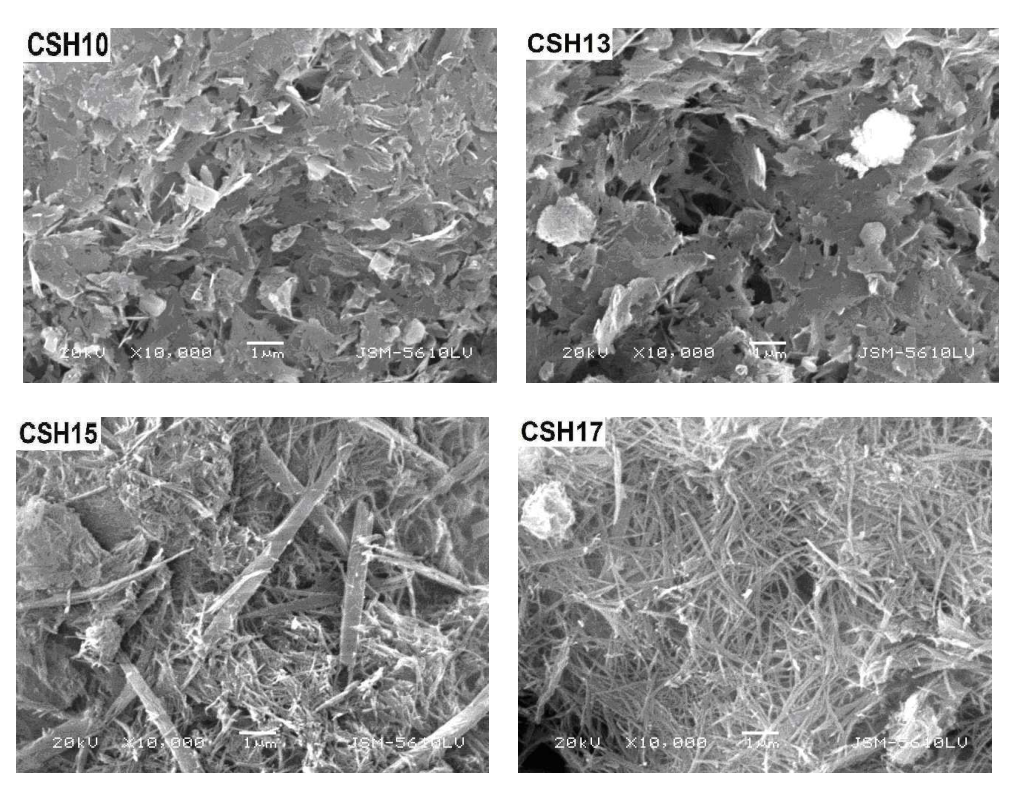
\includegraphics[width=\linewidth]{figures/exp3/lv_csh.png}
  \caption{10000x SEM下, 不同初始钙硅比的\ce{CSH}图像. }
  \label{fig:lv_csh}
\end{figure}

\subsubsection{对粉煤灰的进一步讨论}\label{sec:fa_supp}

我们在图~\ref{fig:15-01-select}观测到粉煤灰维持了球状的样式, 且边界清晰, 表明在我们的实验中, 粉煤灰并没有明显地参与反应. 需要说明的是, 这并不意味着粉煤灰在水泥石中不参与任何反应. 实际上, 在水泥石中, 粉煤灰会参与火山灰反应, 而我们实验中的粉煤灰之所以显示出未进行反应的状态, 是由于火山灰反应速率较慢导致的. 即, 在\SI{7}{\day} 我们终止水化时, 几乎可以认为粉煤灰还没有参与反应.

在宏观层面上, 粉煤灰的掺入会使得水泥石早期的强度降低, 使得后期强度升高. 我们在早期的实验结果(表~\ref{tab:compressive_strength_test})穆庆华的实验结果(表~\ref{tab:strength_fa})有力地表明了这一结论~\cite{mu_fa}. 从表~\ref{tab:strength_fa}中容易发现, 在\SI{28}{\day}前, 掺有粉煤灰的混凝土试块强度都小于不掺粉煤灰的试块的强度, 且强度与粉煤灰掺量呈现负关系; 而在\SI{56}{\day} 及之后, 所有掺粉煤灰的混凝土试块抗压强度均高于不掺粉煤灰的试块的强度, 且强度与粉煤灰掺量呈正关系.

\begin{table}[!t]
  \centering
  \caption{不同粉煤灰掺量、不同天数的水工混凝土抗压强度~\cite{mu_fa}}
  \begin{tabular}{|c|c|c|ccccc|}
    \hline
    \multirow{2}{*}{编号} & \multirow{2}{*}{粉煤灰细度} & \multirow{2}{*}{粉煤灰掺量~(\unit{\percent})} & \multicolumn{5}{c|}{抗压强度~(\unit{\mega\pascal})}                                                                  \\ \cline{4-8}
                          &                             &                                               & \multicolumn{1}{c|}{3d}   & \multicolumn{1}{c|}{7d}   & \multicolumn{1}{c|}{28d}  & \multicolumn{1}{c|}{56d}  & 90d  \\ \hline
    A                     & 12.0                        & 0                                             & \multicolumn{1}{c|}{18.6} & \multicolumn{1}{c|}{28.4} & \multicolumn{1}{c|}{30.5} & \multicolumn{1}{c|}{31.2} & 31.3 \\ \hline
    B                     & 12.0                        & 10                                            & \multicolumn{1}{c|}{17.7} & \multicolumn{1}{c|}{26.5} & \multicolumn{1}{c|}{28.8} & \multicolumn{1}{c|}{32.4} & 33.6 \\ \hline
    C                     & 12.0                        & 20                                            & \multicolumn{1}{c|}{16.4} & \multicolumn{1}{c|}{25.7} & \multicolumn{1}{c|}{27.8} & \multicolumn{1}{c|}{33.2} & 33.6 \\ \hline
    D                     & 12.0                        & 30                                            & \multicolumn{1}{c|}{15.9} & \multicolumn{1}{c|}{25.3} & \multicolumn{1}{c|}{27.1} & \multicolumn{1}{c|}{33.7} & 34.5 \\ \hline
    E                     & 12.0                        & 40                                            & \multicolumn{1}{c|}{14.7} & \multicolumn{1}{c|}{23.6} & \multicolumn{1}{c|}{26.5} & \multicolumn{1}{c|}{34.7} & 35.8 \\ \hline
  \end{tabular}

  \label{tab:strength_fa}
\end{table}

在微观层面上, 我们的实验表明前\SI{7}{\day} 的粉煤灰呈球形, 边界清晰; 随着火山灰反应的进行, 粉煤灰的球形边界会慢慢模糊, 逐渐与周边融为一体.